\outline{1}{Chapter 4}
\chapter{Compensation and Restitution of Post-Stroke Movement Patterns}
\label{cha:armeospring}

In this chapter, I present my study on the ArmeoSpring kinematics data.

\section{ArmeoSpring Overview}
\label{sec:overview}

The ArmeoSpring is a rehabilitation exoskeleton, designed for the purpose of ``functional arm and hand therapy''.\footnote{\label{aowebsite}https://www.hocoma.com/usa/us/products/armeo/armeospring/, last accessed 2/16/2017} 
The device is based on research and development of David Reinkensmeyer at the University of California, Irvine (UCI) and the Rehabilitation Institute of Chicago (RIC). 
Shown in figure \ref{fig:armeo}, the exoskeleton has 7 degrees of freedom (DoF), summarized in table \ref{tab:devicedof}. 
It is attached to the arm by two or three velcro straps. 
The exoskeleton has two springs equipped, at the upper arm and forearm respectively. 
The springs can be adjusted to compensate the gravity force of the arm. 
The lengths of the exoskeleton are adjustable, as well as the strength of the springs. 
There are no motors at any joints, the user has to move actively to control the exoskeleton. 
The user's trunk is mildly constrained by the velcro strap at the upper arm. 

\begin{figure}
	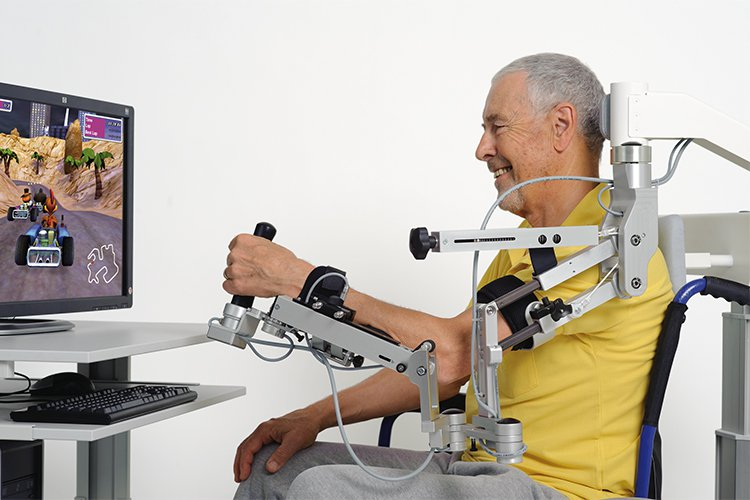
\includegraphics[width=0.5\textwidth]{armeo.jpg}
	\centering
	\caption{ArmeoSpring exoskeleton}
	\label{fig:armeo}
\end{figure}

\begin{table}
	\begin{tabular}{c c c c}
	\hline
	Joint No. & Joint Name & Anatomical Counterpart & Direction \\
	\hline
	1(1) & Inner Shoulder Angle & Shoulder Horizontal Ab-/Adduction & Left/Right \\
	1(2) & Outer Shoulder Angle & Shoulder Horizontal Ab-/Adduction & Left/Right \\
	2 & Upper Arm Angle & Shoulder Flex-/Extension & Up/Down \\
	3 & Elbow Angle & - & Left/Right \\
	4 & Forearm Angle & - & Up/Down \\
	5 & Pro-/Supination Angle & Pro-/Supination & - \\ 
	6 & Flex-/Extension Angle & Wrist Flex-/Extension & - \\
	\hline
	\end{tabular}
	\caption{Degrees of freedom of ArmeoSpring exoskeleton.}
	\label{tab:devicedof}
\end{table}

The device records all joint angles (that is, the joints of the exoskeleton), and calculates the end effector location through a forward kinematics model of the exoskeleton. 
The end effector location then is used to control a cursor on a screen, often displayed vertically in front of the user. 
The stick at the end point is equipped with a force sensor. 
During a training session, the user plays several 2D or 3D games; after a certain game, the user is often presented with performance feedbacks of that game.
Some games have difficulty settings that physical therapists can change at the beginning of a training session.

The ArmeoSpring claims to be the ``preferred therapy choice for arm and hand rehabilitation of the widest range of patients"\footnotemark[\ref{aowebsite}]. 
The lack of motors enables self-initiated movement therapy. 
The device records all joint angles and cursor trajectories, as long as task-specific variables, which helps provide assessments and document patient progress.

\section{Data Collection, Acquisition and Preprocessing}
\label{datacollect}

\subsection{Ladybug pointing test}

The ladybug pointing test (see figure \ref{fig:ladybug}) is a game in which the user tries to catch ladybugs that appear one by one pseudo randomly on a vertical screen in front of the user. 
The game is two-dimensional; the movement along the dimension perpendicular to the screen is ignored. 
To catch the ladybug, the user moves the cursor to its location. After a ladybug is caught, or a certain amount of time if not caught, the ladybug disappears and the next ladybug appears somewhere else. 
We choose this game as a test of performance because we have access to the time and location of the beginning and the end of each movement (if the ladybug is caught).%, namely from the current ladybug to the next.

\begin{figure}
	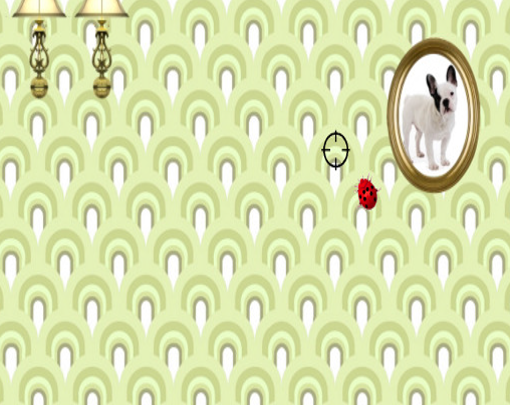
\includegraphics[width=0.5\textwidth]{ladybug.png}
	\centering
	\caption{Ladybug pointing test}
	\label{fig:ladybug}
\end{figure}

This pointing test is scheduled at the beginning and the end of each training session. For the control group (young adults, see below), each session lasts about 20 minutes. 
Two training sessions are scheduled per day in the morning and the afternoon, for 5 consecutive days. 
As a result, each subject has 10 training sessions, 20 ladybug pointing tests. 

For the control group, all games are set to be at the most difficult level. 
Specifically, the ladybug pointing test is set at level 4 in which 48 ladybugs appears sequentially. 
Though the locations of ladybugs seem to be random, they actually appears in a specific sequence at specific locations. 
At level 4, all ladybugs appear on a $6\times8$ grid, in the sequence shown in \ref{fig:48order}. (the sequences at level 1,2 and 3 are also shown.) 

Post-stroke participants received the tests in all 4 levels. 
Each participant might receive different levels through the training.
Figure \ref{fig:diffLevel} shows two examples of how this difficulty setting changes through the training. 
As shown, not every participants share the same pattern, some of them (at least 17 participants) have no difficulty level changes, others have very small changes, as the second example in Figure \ref{fig:diffLevel}. 
The difficulty settings determine the number of targets, the size of workspace (shown in Figure \ref{fig:48order}), and the length of time limit to catch targets.
We report the effects of test difficulty settings in Section \ref{sec:pertaskspace}.

\begin{figure}
	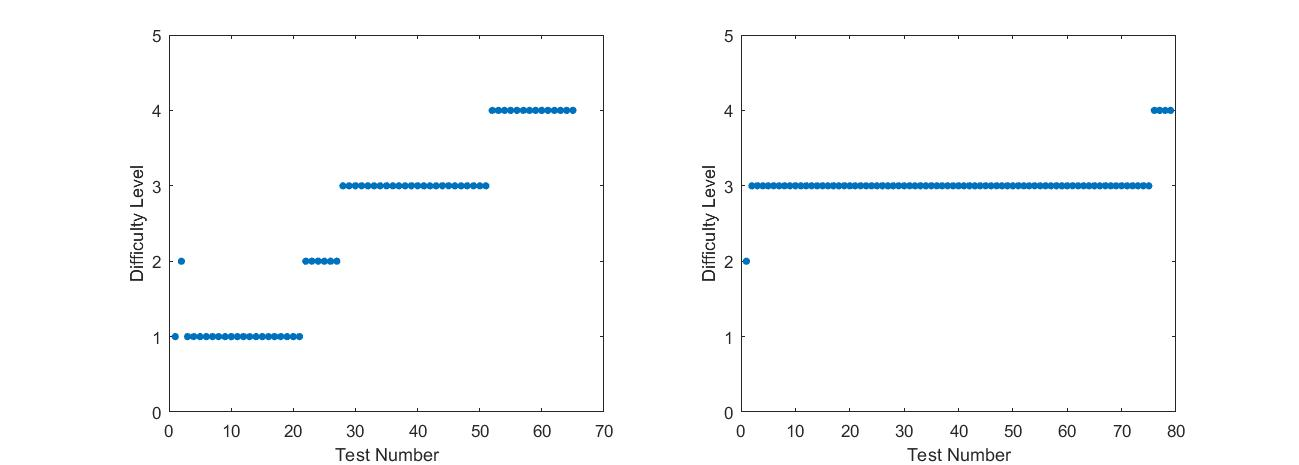
\includegraphics[width=\textwidth]{diffLevel.jpg}
	\centering
	\caption{Example difficulty settings}
	\medskip
	\small 
	\label{fig:diffLevel}
\end{figure}

\begin{figure}
	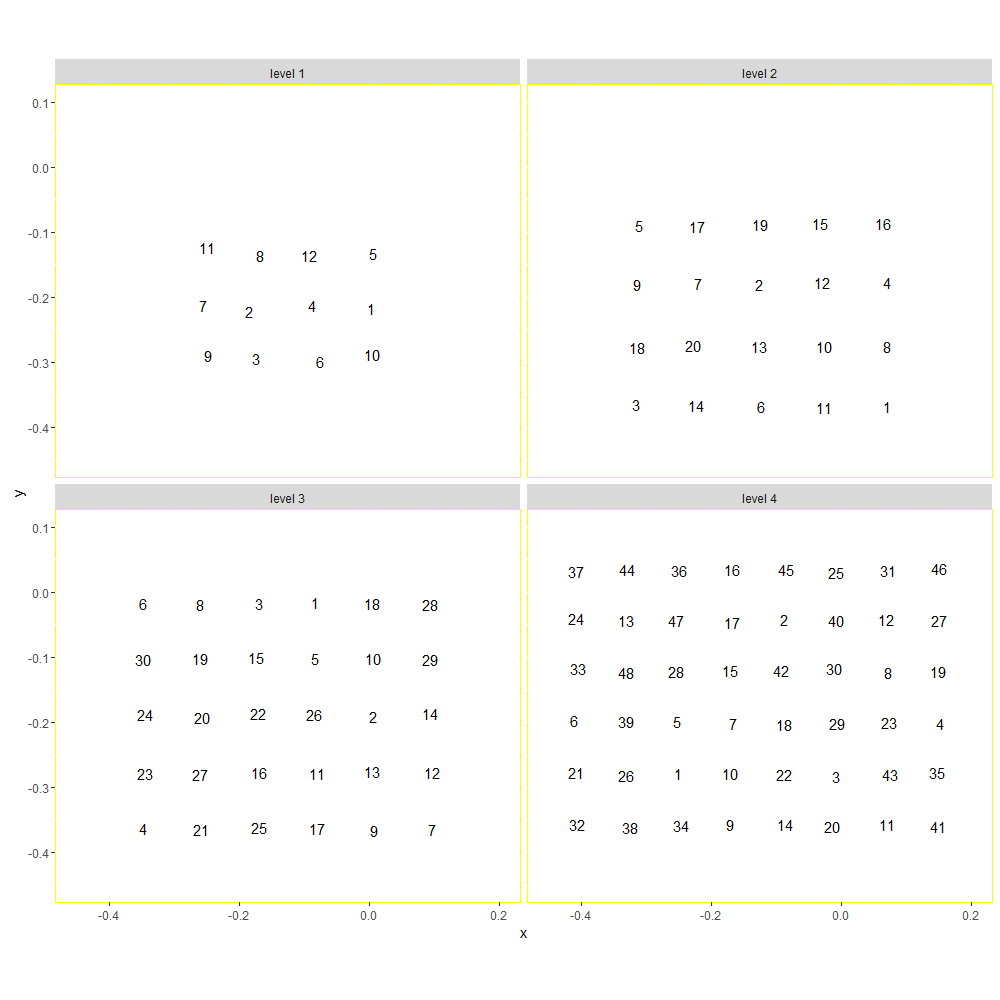
\includegraphics[width=0.8\textwidth]{48order.png}
	\centering
	\caption{Ladybug test difficulty levels and target sequence}
	\medskip
	\small The number indicates the order of the ladybug appearing at that location. The distance between adjacent targets is about 8 cm.
	\label{fig:48order}
\end{figure}

% As a result, the data consists movements that have various starting positions, distances and directions.

\subsection{Participants}

We recruited 11 young (age 23 $\pm$ 2) healthy subjects (7 males) to play the games which are designed for rehabilitation.

Data from post-stroke individuals are collected automatically when participants use ArmeoSpring under guidance from physical therapists. 
Besides ArmeoSpring-aided rehabilitation, participants also receive conventional rehabilitation.
% We have no control over game difficulty, arm length and gravity compensation settings. 
All participants have similar schedules as the control group: there are two training sessions in a day, for four weeks, weekends excluded. Therefore each participant has 40 sessions, 80 ladybug pointing tests.

We have access to data from 53 post-stroke individuals; gender and affected side are balanced, shown in table \ref{tab:demog}. 

\begin{table}[b]
	\begin{tabular}{c c c c c c c c}
	\hline
	Group & No. & Age & Affected Side & Gender & FM(0-66) & Post Stroke Days & No. of Tests\\
	\hline
	Stroke & 53 & 59$\pm$14 & 29L, 24R & 19F, 30M & 25$\pm$9 to 39$\pm$ 14 & 56$\pm$21 & 80 in 4 weeks \\ 
	Control & 11 & 23$\pm$2 & - & 4F, 7M & - & - & 20 in 1 weeks \\
	\hline
	\end{tabular}
	\caption{Participants information}
	\label{tab:demog}
\end{table}


[need relocate]Because participants have different difficulty settings from each other, and each participants may also has various difficulty settings throughout the training, it is important to see the test in different difficulty settings. 
The ladybug test under more difficult settings has larger number of ladybugs to catch, shorter time to catch the bug before it disappears, and bigger the workspace. 
In figure \ref{fig:48order}, configurations of all levels of difficulty are shown. 

[need relocate]The length of the exoskeleton and the strength of the springs also vary, both within and across participants.

We have access to participants' age, gender, affected side, time of stroke and two clinical assessments before and after training: Fugal-Mayer score [ref] (upper extremity) and ARAT [ref]. The distribution of age, gender, affected side and time of stroke is shown in figure \ref{fig:demoData}. Figure \ref{fig:FMARAT} shows FM and ARAT of participants before and after training.

\begin{figure} % /ArmeoSpring Project/user settings/plotDemographic.R
	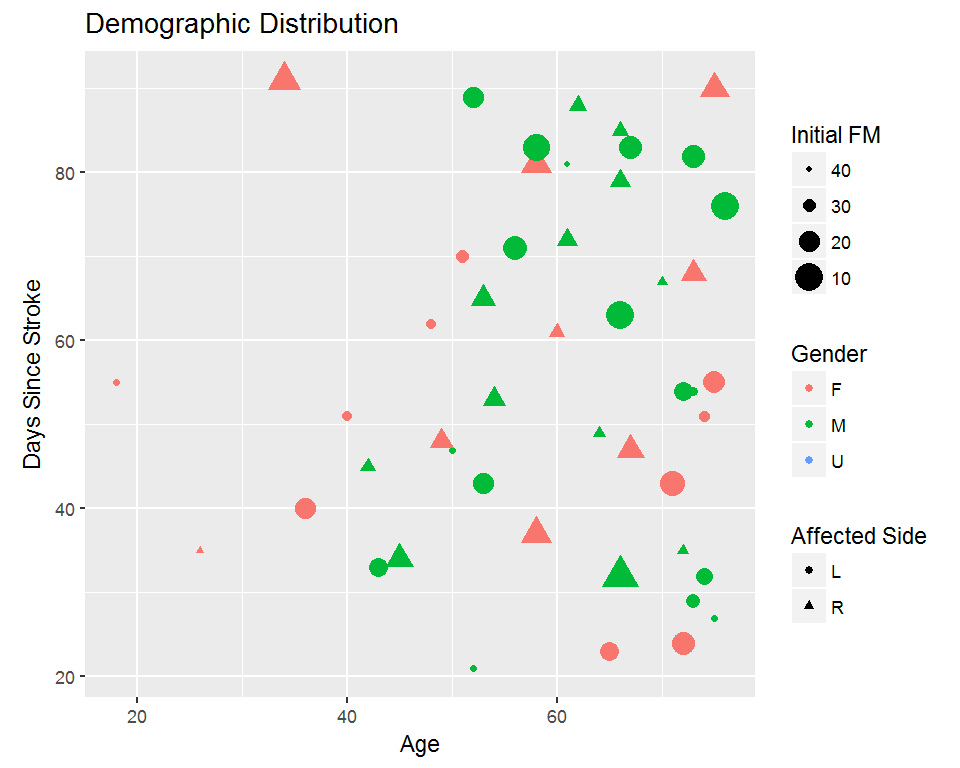
\includegraphics[width=\textwidth]{demoData}
	\centering
	\caption{Demographic Distribution}
	\medskip
	\small 
	\label{fig:demoData}
\end{figure}

\begin{figure} % /ArmeoSpring Project/user settings/plotDemographic.R
	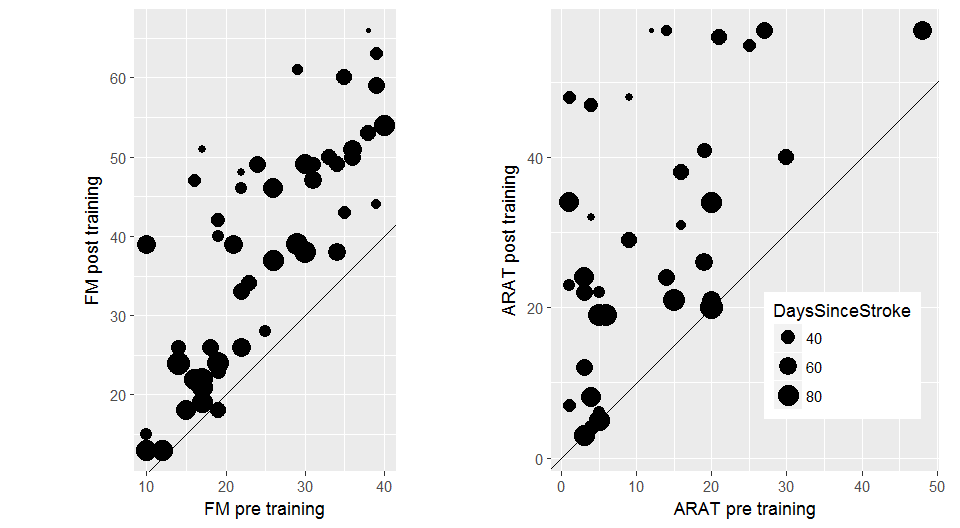
\includegraphics[width=\textwidth]{FMARAT.png}
	\centering
	\caption{FM and ARAT before and after training}
	\medskip
	\small 
	\label{fig:FMARAT}
\end{figure}


\section{Performance in Task Space}\label{sec:pertaskspace}

The kinematics data collected by ArmeoSpring can be viewed as two folds: joint angle trajectories, and end point trajectories. 
However, these two subsets are not independent since the cursor trajectories can be derived through forward kinematics from the joint trajectories. 
Indeed that is how the cursor trajectory data is generated. 
Nevertheless, the cursor trajectories give us valuable insights regarding to each individual's performance.

The ladybug pointing test is a game rendered on a 2D vertical screen. 
To move perpendicularly to the screen has no effect on the test performance. 
In this section, I present the performance of both groups on this 2D task space.

The kinematics data are filtered with a second order Butterworth filter with a cutoff frequency of 5 Hz.

\subsection{Endpoint kinematics performance measures}

Figure \ref{fig:controlTrajExamp} shows an example of cursor trajectories before and after training, from one representative participant [sb=2] in the control group. 
The green star indicates the first ladybug of that test. 
The movement that leads to the catch of the first ladybug is discarded. 
One can immediately see the differences: the trajectories at the last test are more straight and have less over-shooting. 
This will be confirmed in section \ref{}. 
Participants in the control group never miss a target.
In contrast, figure \ref{fig:improverTrajExamp} shows an example from one participant [sb=16] in the post-stroke group. 

We performed a variety of kinematics measures on this set of cursor trajectories data. 
They can be grouped in three groups: 1) Time and duration measure; 2) Curvature and smoothness measure; 3) Movement planning [and/or execution measure]. 

Note that these kinematics measures can reflect both motor learning and motor recovery. There are no obvious way to differentiate the two [ref].

Note that "
However, the end point measurements do not confirm whether such improvement is a genuine motor recovery or due to the appearance of compensation," [Nordin2014]



\begin{figure}
	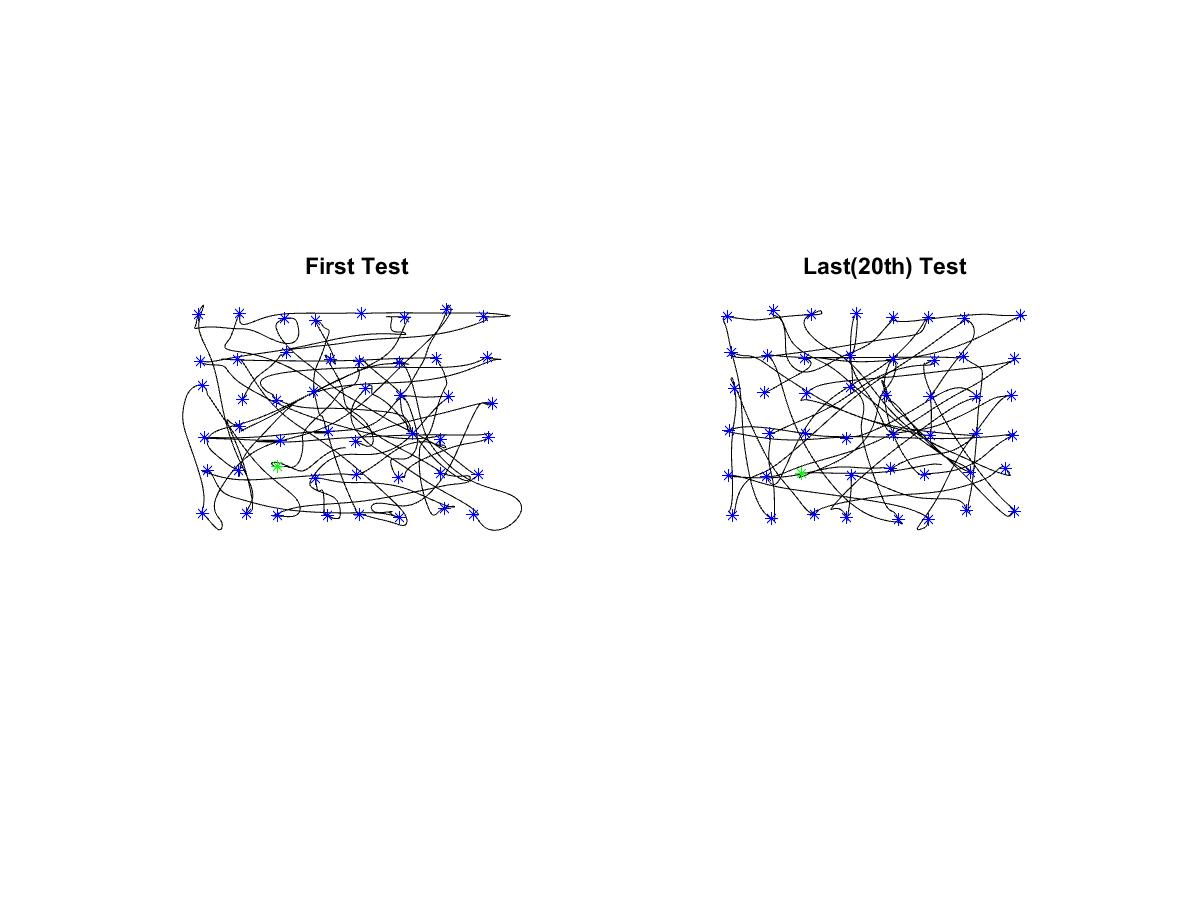
\includegraphics[width=\textwidth]{controlTrajExamp}
	\centering
	\caption{Example trajectories from control group}
	\medskip
	\small The green star is the first target
	\label{fig:controlTrajExamp}
\end{figure}

\begin{figure}
	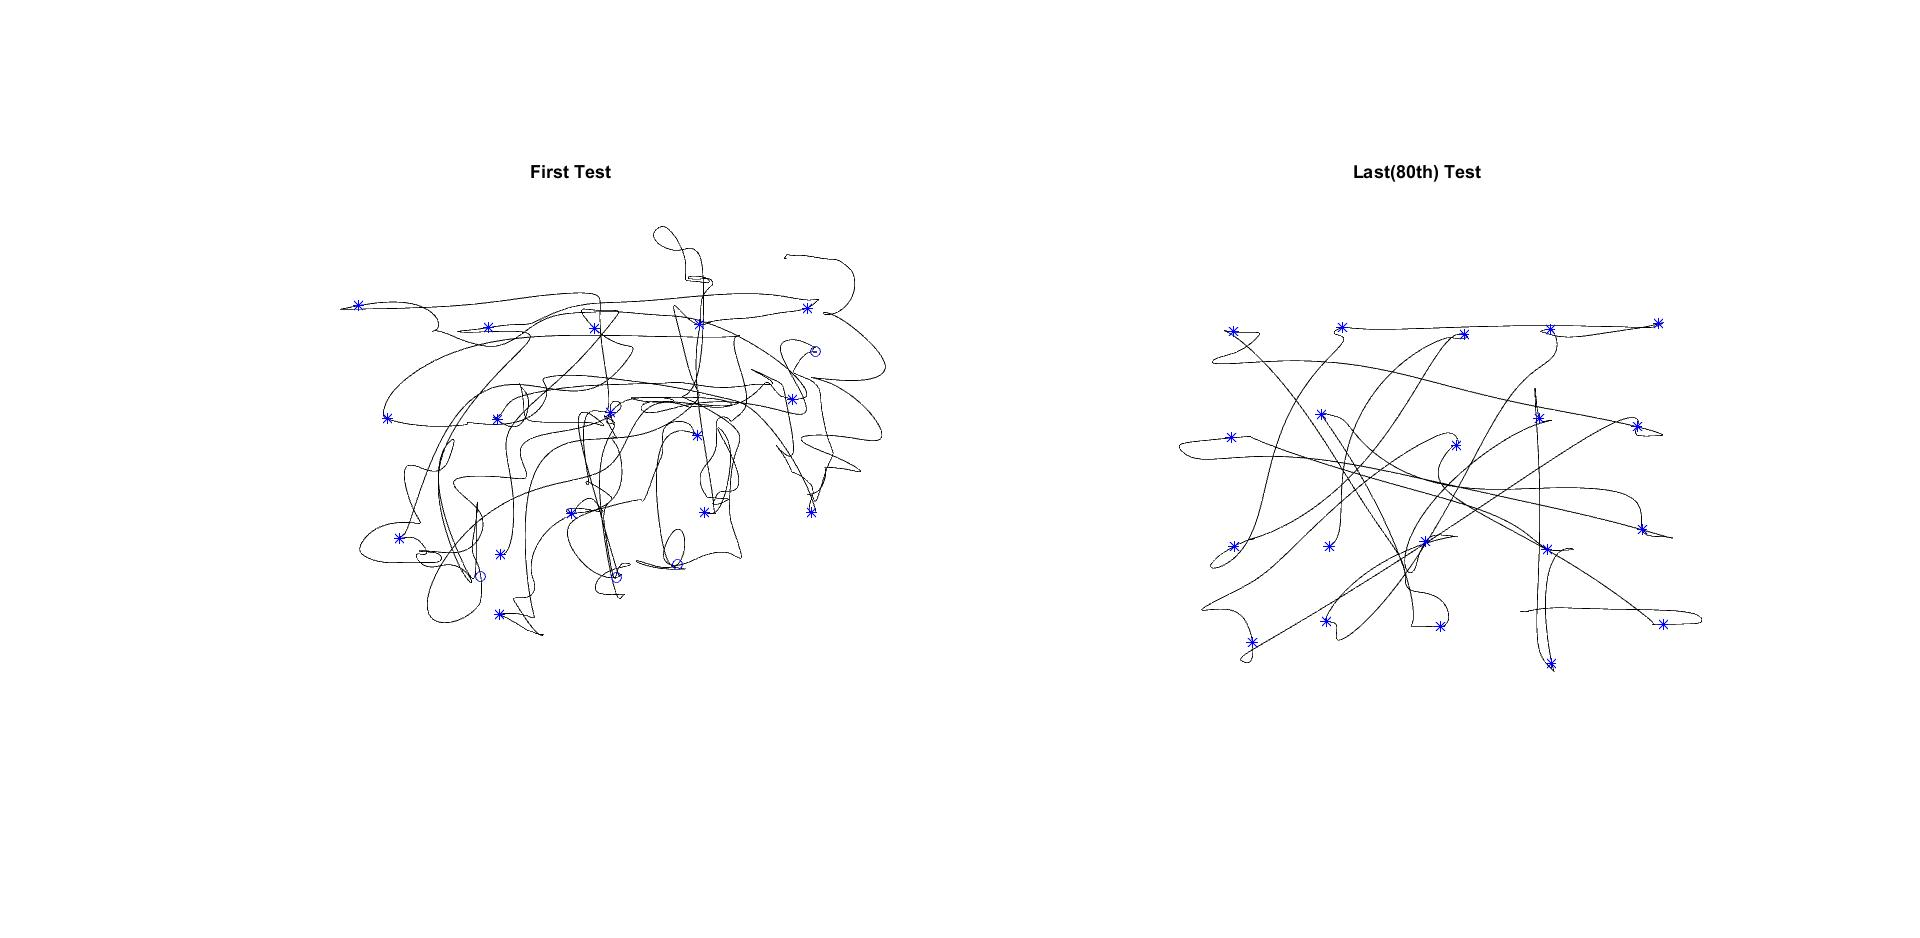
\includegraphics[width=\textwidth]{improverTrajExamp}
	\centering
	\caption{Example trajectories from post-stroke group}
	\medskip
	\small Circles are the locations of the cursor when targets disappear.
	\label{fig:improverTrajExamp}
\end{figure}

\subsubsection{Movement efficacy}
We take the percentage of successful trials as movement efficacy measure \cite{Nordin2014}. 
A successful trial starts from previously caught target and leads to the catch of the next target. 
If the previous target is not caught, then this trial is considered a failure.
Successful rate of a test is the number of successful trials divided by the total number of trials in that test.
The following kinematics measures are only applied to successful trials, if not clarified otherwise.

\subsubsection{Movement planning}
We calculate initial direction deviation and percentage time to peak velocity as a measure of movement planning \cite{Nordin2014}. 
Initial direction deviation is defined as the angle difference between target direction and travel direction (from starting point to peak velocity point).
\cite{Zollo2011} showed that initial direction deviation significantly decreases with robot-aided rehabilitation, and it correlates with Fugal Meyer Assessment Score.
Percentage of time to peak velocity is the percentage of time used from starting point to peak velocity point.
\cite{Chang2007} showed that percentage of time to peak velocity decreases with robot-aided rehabilitation together with conventional rehabilitation.

\subsubsection{Temporal efficiency and movement efficiency}
The time taken to complete a task is expected to reduce with motor learning and recovery.
For each successful trial, we calculate the movement duration, the average velocity (distance between targets divided by movement duration) and the average tangential velocity (total length of traveled path divided by movement duration).
Following these definitions, the ratio of average tangential velocity to average velocity is exactly the path-length ratio mentioned below.

To account for failed trials, we also use test completion time to measure temporal efficiency. 
Test completion time is the total time period used for the entire test.
To compare across different test levels, we normalize test completion time by the number of targets in that test.

The efficiency of movement is measured by path-length ratio, which is the total length of traveled path divided by the distance between targets \cite{Cirstea2000}. 
The minimum value of path-length ratio is one, achieved when the cursor travels along a straight line. 
Similar measurements are area enclosed by the straight line and the trajectory \cite{Kim16 from Nordin2014}, and maximum or mean deviation of the trajectory from the straight line \cite{Colombo61 from Nordin2014}. 
We only report path-length ratio because the other two measures produced similar results.

\subsubsection{Movement smoothness}

Post-stroke participants usually present jagged movements, appearing as a series of short and rapid sub-movements \cite{Rohrer1 from Nordin2014}.
The number of peaks in the velocity profile is an natural measure of jagged movements, as seen in many studies \cite{}. 
However, the number of peaks of a certain velocity profile depends greatly on how the data is preprocessed, for example, date preprocessed with different filter can report different number of peaks.

[] proposed a minimum jerk model of human reaching movement.
We used a dimensionless jerk definition \cite{HOgan92 in Nordin2014} to measure movement smoothness, because it does not depend on movement duration and distance.

\subsection{Results}

Participants in the control group achieved 99.86\% successful trials, with at most 3 failed trials in about 1000 trials for each individual.
Participants in the stroke group achieved lower successful rate. 
21 out of 52 participants keep a high successful rate ($>$90\%) through all tests;
23 participants show significant improvement;
9 participants have relatively low successful rates ($\sim$80\%) that depend on the test difficulty level setting (see \ref{}).
Figure \ref{fig:efficacy} shows examples of participants' successful rate.

Because of differences in test difficulty settings across different tests, successful rate by itself is not sufficient to evaluate participants' learning or recovery. 

\begin{figure}
	\centering
	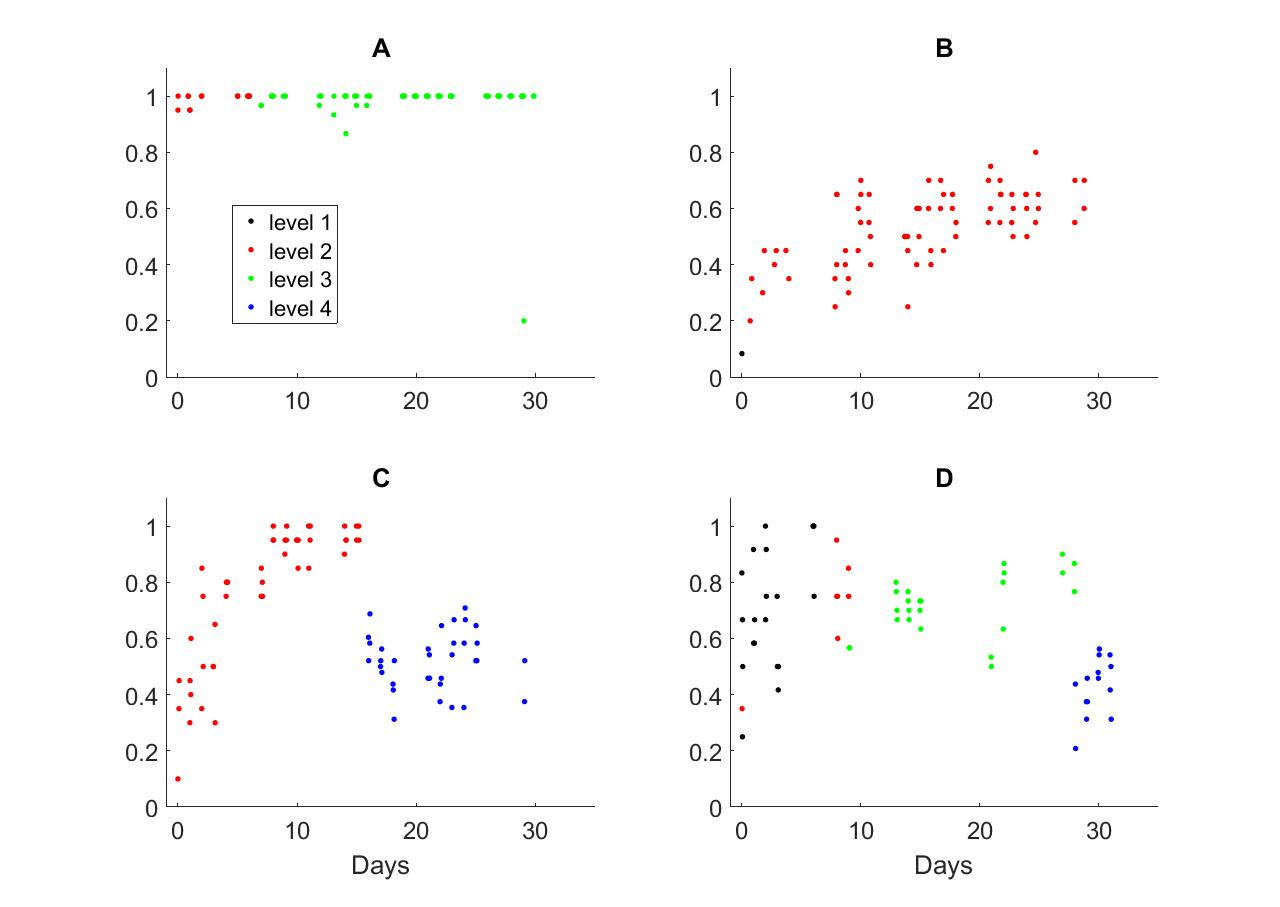
\includegraphics[width=0.8\linewidth]{figures/efficacy}
	\caption[Movement efficacy measured by successful rate.]{Movement efficacy measured by successful rate. Different color indicates difficulty settings. Panel A shows a participant who keeps a high successful rate; Panel B shows a participant who significantly improves; Panel C and D show participants whose successful rates depend on difficulty levels. Shaded area represents standard deviation.}
	\label{fig:efficacy}
\end{figure}

As shown in figure \ref{fig:planning}, Participants in the control group show significant improvement in initial direction deviation and percentage of time to peak velocity. 
In comparison, post-stroke participants improve much slower. 

\begin{figure}
	\centering
	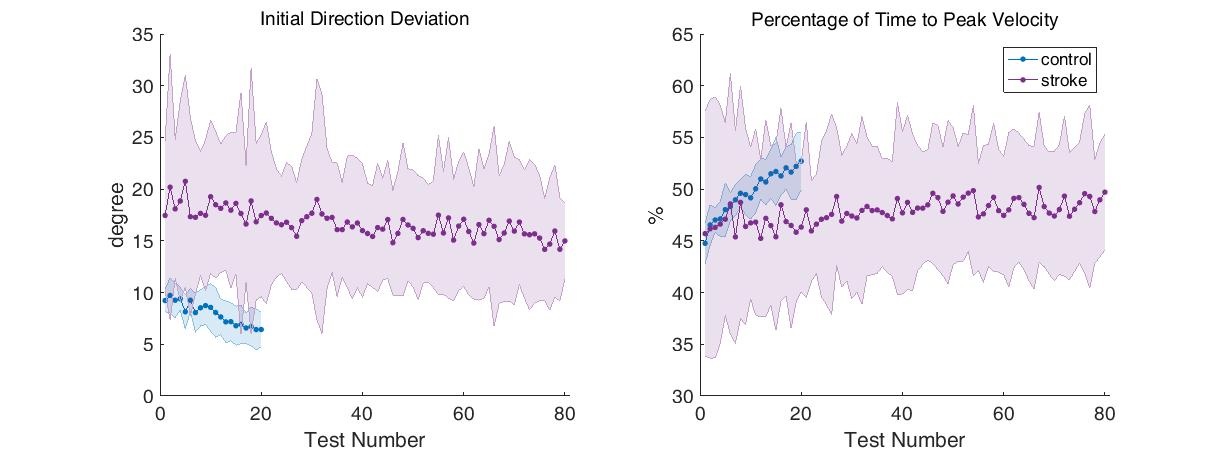
\includegraphics[width=\linewidth]{figures/planning}
	\caption[Movement planning measured by initial direction deviation and percentage of time to peak velocity.]{Movement planning measured by initial direction deviation and percentage of time to peak velocity. Shaded area represents standard deviation.}
	\label{fig:planning}
\end{figure}

Participants in both groups show a decrease in averaged movement duration, as shown in figure \ref{fig:efficiency}.

\begin{figure}
	\centering
	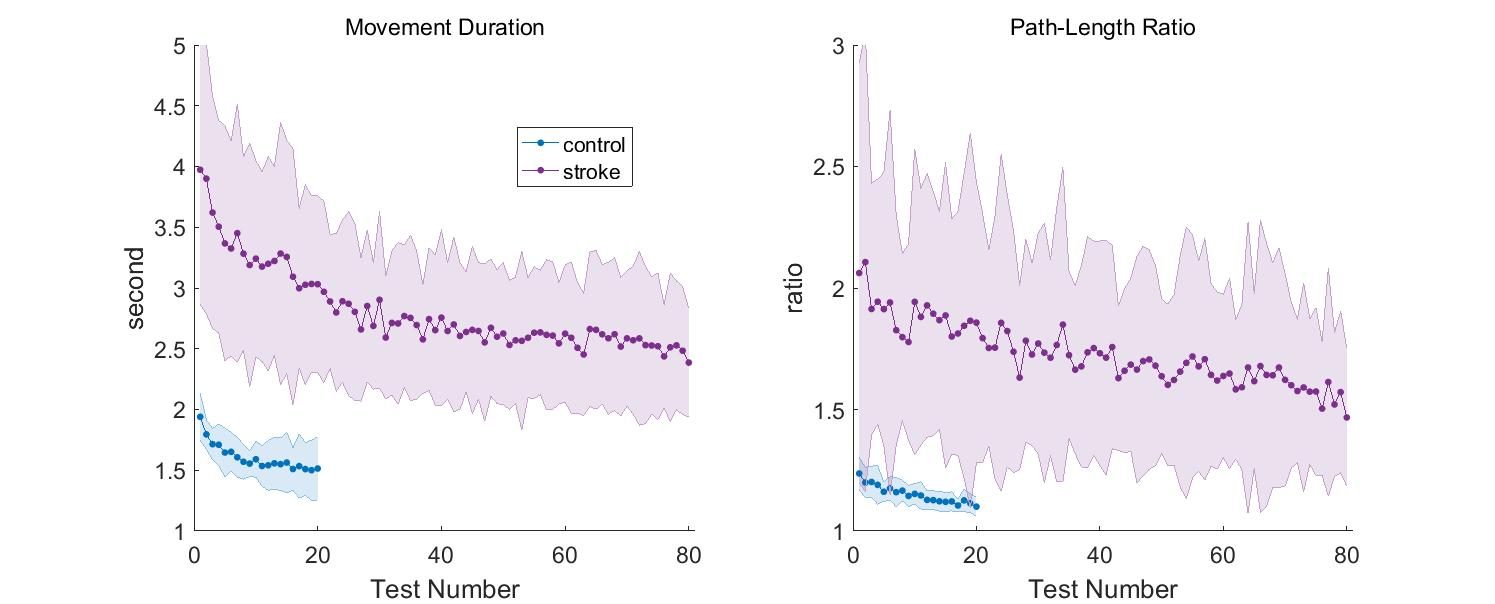
\includegraphics[width=\linewidth]{figures/efficiency}
	\caption[Averaged movement duration and path-length ratio]{Averaged movement duration and Averaged path-length ratio both decreases through the training.}
	\label{fig:temporalefficiency}
\end{figure}



\subsection{Performance of the Control Group}

In this section, I present the performance of the control group as measured by methods introduced in previous section. The main purpose is to estimate a baseline performance learning curve, to be compared, as a standard, with stroke group. Overall, participants in the control group show less cross-subject variance, comparing to the stroke group \ref{}. 

\textit{Method and Notations.} For each kinematics measure (take velocity $VEL$ for example), I first calculate the average $VEL$ and standard error within each test $\sigma_{VEL}$, and then calculate the group average $VEL_\textsf{group} = \textsf{mean}(VEL)$ and standard deviation $\sigma_{VEL_\textsf{group}} = \textsf{std}(VEL)$ aross participants.

\subsubsection{Tangential velocity}
The tangential velocity ($VEL_\textsf{control}$) and average speed ($SPE_\textsf{control}$) of the control group is shown in figure \ref{fig:velControlAve}. Speed and velocity are highly correlated with each other, but the gap between them decreases slightly in time (which is also shown by path ratio in \ref{}). Note that $VEL$ increases faster at the beginning, and slows down at later stage of training. This feature is also shown in the following measures.

\begin{figure}
	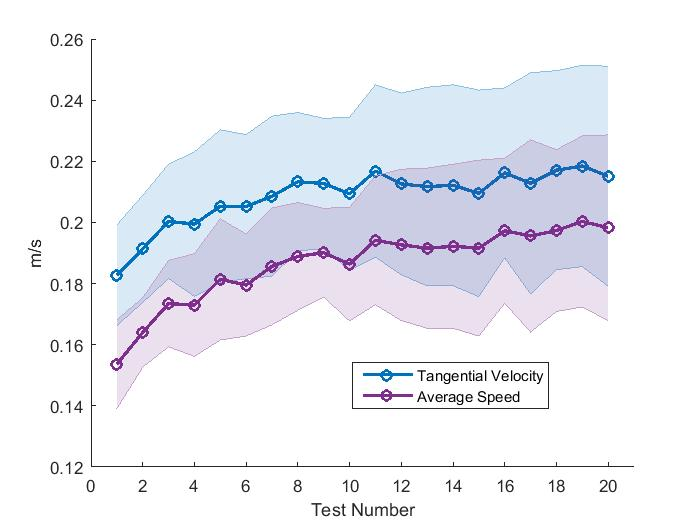
\includegraphics[width=0.7\textwidth]{velControlAve.jpg}
	\centering
	\caption{Tangential Velocity and Average Speed of control group}
	\medskip
	\small The shade represents standard deviation.
	\label{fig:velControlAve}
\end{figure}

\subsubsection{Smoothness}
We choose path ratio (pr), number of peaks (nop) and normalized jerk (nj) as a measure of smoothness. The group average data is shown in figure \ref{}. Note that the variability across subject is not very big. nop can be very well captured by linear mixed effect model. exponential model is inferior. 

\subsection{Performance of the Stroke Group}

Compared with the control group, data from the stroke group present much more variablity, both within and across participants. The data is made more complex by the fact that each participant may have different difficulty settings through out the training. So it is important to investigate the stroke group in more detail than the control group.






\section{Joint Coordination}

\subsection{Joint Angle Data Overview}
Although the device has seven degrees of freedom (as shown in \ref{tab:devicedof}), the first two degrees of freedom both contributes to shoulder horizontal abduction/ adduction movement, therefore they essentially degenerate into one degree of freedom.

The joints of the device do not represent anatomical joints, nevertheless, three device joints can be mapped to anatomical joints directly: Shoulder Angle $\,\to\,$ Shoulder Horizontal Ab-/Adduction, Upper Arm Angle $\,\to\,$ Shoulder Flexion/ Extension, Wrist Flexion/ Extension Angle $\,\to\,$ Wrist Flexion/ Extension. Pro-/Supination Angle of the device is not the anatomical pro-/supination angle, though they are highly correlated.


\subsection{[to-write](Attempt to)Get Joint Angles from Machine Joint Angle Recordings }
\subsection{[to-write]Pros and Cons of Dimensionality Reduction Method for Synergy Abstraction}
\subsection{[to-write]Relationship with Performance in Task Space}
